\documentclass[11pt]{article}

\usepackage[T1]{fontenc}
\usepackage[utf8]{inputenc}
\usepackage{lmodern}
\usepackage{amsmath}
\usepackage[a4paper,margin=2.5cm]{geometry}
\usepackage{booktabs}
\usepackage{longtable}
\usepackage{array}
\usepackage{graphicx}
\usepackage{fancyvrb}
\usepackage{xcolor}
\usepackage{titlesec}
\usepackage{enumitem}
\usepackage[colorlinks=true,linkcolor=blue!50!black,citecolor=blue!50!black,urlcolor=blue!50!black,bookmarksnumbered=true]{hyperref}
\usepackage{caption}
\usepackage{parskip}
\usepackage{seqsplit}
\newcommand{\bcode}[1]{\texttt{\seqsplit{#1}}}

\newcommand{\code}[1]{\texttt{\detokenize{#1}}}
\newcolumntype{L}[1]{>{\raggedright\arraybackslash}p{#1}}

\definecolor{codebg}{gray}{0.95}
\fvset{fontsize=\scriptsize,frame=single,rulecolor=\color{gray!50},xleftmargin=0.5em,xrightmargin=0.5em}

\title{\textbf{LDscnR-multi}\\[0.3em]\Large A User Manual}
\author{}
\date{\today}

\begin{document}
\maketitle

\begin{abstract}
\noindent
This manual explains how to run LD-aware association scans with
\code{LDscnR-multi}, either for one dataset or for hundreds in a batch.
The workflow uses the \code{LDscnR} R package to group correlated markers
before testing, report candidate regions, and compare discovery counts with
structure-aware null analyses. Examples use full-genome three-spined
(117 individuals, 790{,}578 markers) and nine-spined stickleback
(149 individuals, 1{,}195{,}557 markers) panels. Smaller two-chromosome
datasets are provided for a quick first run.
\end{abstract}

\tableofcontents
\newpage

% =============================================================================
\section{Introduction}
% =============================================================================

\code{LDscnR-multi} is a script-based workflow, not a second R package.
Install \code{LDscnR} from GitHub, then use this repository's scripts to
analyse one dataset or a collection of dataset folders. Each dataset keeps
its own inputs and results; a batch run also produces a combined summary.

On the machines used for the examples, a full run took approximately
\textbf{12 minutes for 790{,}578 markers} (three-spined stickleback) and
\textbf{24 minutes for 1{,}195{,}557 markers} (nine-spined stickleback).
These are measured examples, not promised runtimes: marker density, memory,
processor speed, permutation count and plotting choices matter. The
association step is comparatively quick because \code{emmax_fast()} reuses
the fitted relationship model while scanning markers or reduced units;
Stage-1 LD calculations and the floor profile account for much of the
remaining time.

\subsection{What problem this pipeline solves}

A genome scan for markers associated with a phenotype (or an ecological
gradient) faces a structural problem: markers in linkage disequilibrium (LD)
with each other are not independent tests. Naively testing every marker
treats a single underlying signal --- one causal region --- as though it were
dozens or hundreds of separate discoveries, inflating both the apparent
strength of a hit and the multiple-testing burden of the whole scan.

\code{LDscnR}'s answer is a two-stage design, and \code{LDscnR-multi} runs
both stages, per dataset:

\begin{itemize}
  \item \textbf{Stage A} (\code{run_stage_A()}): genotypes + a marker map +
  a phenotype are turned into association p-values, using EMMAX (a mixed
  model correcting for relatedness/population structure via a genomic
  relationship matrix, GRM). Two independent \emph{arms} are computed (see
  Section~\ref{sec:stage-a}):
  \begin{itemize}
    \item \code{unit} --- one test per LD-cluster (a ``unit''), collapsing
    correlated markers into one representative test;
    \item \code{simes} --- one p-value per individual marker, aggregated up
    to its cluster via Simes' method.
  \end{itemize}
  \item \textbf{Stage B} (\code{run_stage_B()}): takes Stage A's cluster-level
  results, or aggregates marker-level p-values from Stage A or an external
  method such as LFMM. It identifies significant LD-clusters and assembles
  nearby significant clusters into reported \emph{regions}.
\end{itemize}

Everything else in this manual --- the LD-decay report, the structure-alignment
diagnostic, the floor profile, the Manhattan plots --- exists to support,
calibrate, or visualise these two stages.

\subsection{Relationship to \code{LDscnR} and \code{LDscnR-paper}}

\code{LDscnR} supplies the clustering, association and outlier functions.
\code{LDscnR-multi} organises them into a repeatable workflow for one or
many datasets. Its example data come from the stickleback analyses in the
LDscnR study; you do not need the manuscript or its analysis scripts to
follow this manual.

\subsection{Design philosophy: receipts, not blind reruns}

Every stage records its inputs and settings and skips recomputing when
nothing has changed (Section~\ref{sec:receipts}). This helps with both a
single dataset and large batches.

% =============================================================================
\section{Key concepts}
\label{sec:concepts}
% =============================================================================

This section defines every piece of pipeline-specific vocabulary used later.
Skip it if you already know what an LD-complexity-reduction cluster, a
\code{size_floor}, or a floor profile is.

\subsection{Stage 1 clustering: units and \texttt{core\_snp}}

Before any association test runs, \code{LDscnR}'s
\code{ld_complexity_reduction()} groups markers into clusters (called
\emph{units} downstream) purely from genotype LD, with no phenotype
involved. Two markers land in the same cluster only if the pairwise LD
between them, and everything along a chain connecting them, clears a
threshold $\rho$ (this repository's default \code{cr_rho = 0.5}). Each
cluster gets one representative marker, its \code{core_snp}, which never
changes as long as the clustering itself is unchanged --- this is what makes
\code{core_snp} the right key for comparing clusters across a floor profile
(Section~\ref{sec:floor-profile}), where a cluster's position index
(\code{unit_id}) is \emph{not} stable.

\subsection{\texttt{ld\_w}: local LD support}
\label{sec:ldw-concept}

\code{ld_w} (reported at $\rho = 0.95$ as \code{ld_w_095} throughout this
pipeline's output) is a per-marker statistic answering: ``how much local LD
support does this marker have?'' It comes from fitting a decay curve
$r^2 \sim b + (c-b)/(1+a\cdot d)$ to how LD falls off with distance $d$ on
each chromosome, then asking, for each marker, how far its own local LD
extends before dropping below the $\rho$ threshold. A marker sitting inside
a large block of mutually correlated markers (e.g.\ an inversion, or a
region of suppressed recombination) has high \code{ld_w}; a marker in an
isolated, low-LD stretch of the genome has low \code{ld_w}. It is
\emph{not} a test statistic and carries no p-value of its own --- it is a
structural, genotype-only property of the marker's neighbourhood, reported
alongside every association result as context (Section~\ref{sec:ld-decay}),
and plotted directly as an alternative Manhattan-plot axis
(Section~\ref{sec:manhattan}).

\subsection{\texttt{size\_floor}: the minimum tested cluster size}
\label{sec:size-floor-concept}

Not every Stage-1 cluster is tested. \code{size_floor} is the minimum
number of markers a cluster must contain to be tested at all; smaller
clusters are skipped, never assigned a p-value. This reduces the number of
tests and makes the minimum support required of a tested cluster explicit.
The pipeline requires at least two markers per tested cluster. Small
clusters can nevertheless contain real signals; raising the floor trades
genomic coverage for a smaller, more concentrated test set
(Section~\ref{sec:floor-profile}).

\subsection{Regions: assembling significant units}

A significant unit does not stand alone in the reported output. Once Stage B
has decided which units clear the significance threshold, it assembles
physically nearby significant units into a \emph{region} (one row of
\code{region_table.csv}, Section~\ref{sec:stage-b}). Two assembly modes
exist: \code{stage2_discovered} (the default --- a second round of
\code{LDscnR}'s own clustering, at a possibly different LD threshold, run on
just the significant units) and \code{physical} (a simpler gap-merge of
significant units' own physical spans). This manual's example output uses
the default.

\subsection{Permutation nulls and why permutation function matters}

Calibration repeats the association analysis with surrogate phenotypes to
see how many discoveries could arise without the observed
phenotype--genotype relationship. \emph{How} the surrogate is constructed matters:
shuffling individuals directly, ignoring population structure, can break the
very structure a mixed model is meant to account for. \code{LDscnR-multi}
therefore requires every dataset with an EMMAX phenotype scan to supply its own \code{perm_fun.R}
(Section~\ref{sec:dataset-contract}) rather than assuming a generic shuffle
is safe.

% =============================================================================
\section{Installation and setup}
% =============================================================================

Install the validated \code{LDscnR} revision from GitHub, then download
this repository. The first command needs internet access; subsequent
analyses run from local files. The validated revision is recorded in
\code{R/00_config.R} as \texttt{LDSCNR\_PIN\$sha}.

\begin{Verbatim}
install.packages("remotes")               # once, if needed
remotes::install_github("genomeinsights/LDscnR@2fc1d44a2552")
library(LDscnR)
\end{Verbatim}

\code{LDscnR-multi} itself is not installed as a package. From its
repository directory, either source its scripts in R:

\begin{Verbatim}
library(LDscnR)
for (f in sort(list.files("R", pattern = "\\.R$", full.names = TRUE))) source(f)
run_dataset("examples/3sp_chr1_chr4")
\end{Verbatim}

or, from the shell, \code{run_batch.R} does both steps for you and then runs
the pipeline over one or more dataset folders:

\begin{Verbatim}
Rscript run_batch.R examples/3sp_chr1_chr4 examples/9sp_chr19_chr20
Rscript run_batch.R examples/                 # every subfolder with an input/
\end{Verbatim}

\subsection{The \code{LDscnR} version pin}
\label{sec:ldscnr-version}

The pipeline checks the GitHub commit recorded in the installed package,
not merely its version number. If it does not match the validated revision,
the run stops before processing a dataset. This prevents a large batch
from mixing results obtained with different package code. Reinstall the
revision shown above when that happens. Developers working from a local
checkout may set \code{LDSCNR_DEV_LOAD_ALL=1} before using
\code{run_batch.R}; that mode loads the checkout and checks its source
instead. Ordinary users need neither a local \code{LDscnR} checkout nor
\code{devtools}.

% =============================================================================
\section{How many markers should be included?}
\label{sec:marker-density}
% =============================================================================

For most applications, we suggest starting with a well-distributed panel
of no more than approximately \textbf{one million filtered markers}. This
is a practical target, not a biological or software limit. The default
floor profile ultimately tests only the larger LD clusters, so adding
many densely packed markers can increase LD calculations and plotting
time without adding many distinct tests. The examples show that even a
1.2-million-marker panel is feasible, but it takes longer and uses more
memory than the 790{,}578-marker panel.

If the starting panel is substantially denser, thin it \emph{before}
building the input files. First apply the study's usual missingness, MAF
and quality filters. Then use a recorded random seed to sample markers
across every chromosome and across short physical bins within chromosomes,
limiting very dense bins while retaining several markers per bin. Set bin
width and per-bin sampling quotas from the genome length and desired total
so that broad coverage is maintained; do not select markers using their
phenotype association or keep only one marker from each LD cluster, which
would defeat the cluster-based test. Apply the same selected marker IDs and
order to \code{genotypes.rds}, \code{map.rds} and any
\code{external_pvalues/} vectors. Record the filter, seed, binning rule and
retained marker count.

Thinning \emph{can} change LD estimates, cluster sizes and discoveries.
An outlier region represented by too few retained markers may disappear,
whereas additional markers in an unthinned panel could have made its LD
pattern testable. Therefore, when possible, compare the floor profile and
main candidate regions on one representative denser dataset before
applying the chosen thinning rule to hundreds of datasets. The one-million
target should never be interpreted as proof that denser data cannot reveal
additional regions.

% =============================================================================
\section{Dataset folder contract}
\label{sec:dataset-contract}
% =============================================================================

Every dataset is one self-contained folder. Nothing about it is registered
anywhere else; passing its path to \code{run_dataset()} is the only thing
that ties it into the pipeline.

\subsection{\code{input/} --- what you provide}

\begin{longtable}{@{}L{3.8cm}L{2.2cm}L{8.3cm}@{}}
\toprule
\textbf{File} & \textbf{Required?} & \textbf{Contents} \\
\midrule
\endhead
\code{genotypes.rds} & required & An $n \times m$ numeric dosage matrix
  (values in $[0,2]$, \code{NA} allowed), individuals in rows
  (\code{rownames} = individual IDs), markers in columns (\code{colnames} =
  marker IDs). \\
\code{map.rds} & required & A \code{data.table}/\code{data.frame} with
  columns \code{marker}, \code{Chr}, \code{Pos}. \texttt{map\$marker} must
  equal \code{colnames(genotypes)}, in the same order. \\
\code{phenotype.rds} & only for Stage A & A named numeric vector (names =
  \code{genotypes}' rownames), or a one-column data frame with those row
  names. \\
\code{perm_fun.R} & required for Stage A & Plain R defining
  \code{perm_fun(b, y)}, returning one permuted copy of phenotype \code{y}
  for permutation index \code{b}. There is deliberately no generic default
  (see Section~\ref{sec:concepts}); see the real example below. \\
\code{population.rds} & only for the structure-alignment diagnostic &
  Named vector, individual $\to$ population ID. \\
\code{structure_group.rds} & optional & Named vector, individual $\to$ a
  coarser sampling group (locality, lineage, \ldots). Defaults to
  \code{population.rds} when absent; this is the grouping a permutation is
  actually restricted within. \\
\code{config.R} & optional & Plain R assigning any \code{DEFAULTS} name from
  \code{R/00_config.R} (Section~\ref{sec:config-reference}) to override it
  for this dataset only, e.g.\ \code{cr_rho <- 0.35}. \\
\bottomrule
\end{longtable}

\code{external_pvalues/} is a second, optional top-level folder: one
\code{.rds} per extra p-value engine, each a \emph{named} numeric vector
(names = \texttt{map\$marker}). The file name, minus \code{.rds}, becomes the
engine name --- \code{external_pvalues/lfmm.rds} is run through Stage B as
engine \code{lfmm}. This is how \code{LDscnR-multi} stays engine-agnostic:
Stage B does not care whether a p-value came from its own Stage A or from an
entirely different method, as long as it is one p-value per marker.

\subsubsection{A real \texttt{perm\_fun.R}}

The example's permutation function is shown below. The phenotype
(ecotype) is constant within a population, so an
individual-level shuffle would create within-population variation that
never exists in the real data; this shuffle instead reassigns \emph{which}
population gets which value, restricted to populations sharing the same
locality:

\VerbatimInput[firstline=12,lastline=23,fontsize=\tiny,frame=single]{../examples/3sp_chr1_chr4/input/perm_fun.R}

\subsubsection{What \code{genotypes.rds}/\code{map.rds}/\code{phenotype.rds} actually look like}

From \code{full_runs/3sp_full} (117 individuals $\times$ 790{,}578 markers
--- the corner shown below happens to be identical to the small worked
example's own copy, since both start from the same Chr1):

\begin{Verbatim}
> g <- readRDS("input/genotypes.rds"); g[1:4, 1:4]
      Chr1:2480 Chr1:2492 Chr1:2493 Chr1:2494
ind_1  0.007751  0.015384  0.058822  1.000001
ind_2  0.003891  0.003891  0.007751  0.999986
ind_3  1.000000  1.000000  1.000014  0.003891
ind_4  0.000244  0.038510  0.003891  1.000000

> m <- readRDS("input/map.rds"); head(m)
     marker  Chr  Pos
1 Chr1:2480 Chr1 2480
2 Chr1:2492 Chr1 2492
3 Chr1:2493 Chr1 2493
...

> p <- readRDS("input/phenotype.rds"); head(p)
ind_1 ind_2 ind_3 ind_4 ind_5 ind_6
    0     0     0     0     0     0
\end{Verbatim}

\subsection{\code{cache/} and \code{output/} --- what the pipeline writes}

Both are gitignored and fully regenerable: delete either one and rerun to
get it back (subject to the receipt system re-deciding what actually needs
recomputing, Section~\ref{sec:receipts}). \code{cache/} holds the GDS
genotype file, the LD-decay fit, the Stage-1 clustering, and the GRM ---
everything that depends only on genotypes, never on a phenotype. Note there
is deliberately no \code{cache/edge_lists/}: at full-genome marker density a
single chromosome's raw pairwise edge list can run several gigabytes, so it
is never persisted to disk --- every consumer rebuilds it from the GDS file
on the fly, one chromosome at a time, and discards it immediately after use.
\code{output/} is described stage by stage in Section~\ref{sec:stages}, and
summarised as a full tree in Appendix~\ref{sec:appendix-tree}.

% =============================================================================
\section{Running the pipeline}
\label{sec:running}
% =============================================================================

The typical entry point is \code{run_dataset(dataset_dir)}, which runs
every applicable stage, in order, for one dataset. The two-chromosome worked
examples under \code{examples/} are the right thing to point this at first
--- a full genome panel like this manual's own \code{full_runs/3sp_full} (20
chromosomes, 790{,}578 markers) genuinely takes minutes per stage, not
seconds: a real, from-scratch, single-machine timed run of
\code{full_runs/3sp_full} took about 6.3 minutes for Stage 1, 3.8 minutes for
the floor profile, under 15 seconds each for the LD-decay report, the
structure-alignment diagnostic, Stage A, and each Stage B engine, and about
35 seconds per Manhattan figure --- roughly 12 minutes end to end on this
790{,}578-marker panel; the nine-spine panel (1{,}195{,}557 markers) took
about 24 minutes. Section~\ref{sec:receipts} covers why a second call on an
unchanged dataset is nonetheless cheap:

\begin{Verbatim}
run_dataset("examples/3sp_chr1_chr4")

result <- run_all(c("examples/3sp_chr1_chr4", "examples/9sp_chr19_chr20"))
result$summary            # one row per (dataset, engine)
result$alignment_summary  # one row per dataset with input/population.rds
\end{Verbatim}

Internally, \code{run_dataset()} executes the following steps, each gated by
its own receipt (so a repeat call after a partial change re-runs only what
actually needs it):

\begin{enumerate}
  \item \textbf{Stage 1} (Section~\ref{sec:stage1}) --- genotype-only LD
  clustering, always runs.
  \item \textbf{LD-decay report} (Section~\ref{sec:ld-decay}) --- always
  runs, genotype-only, no recomputation (just writes what Stage 1 already
  computed).
  \item \textbf{Structure-alignment diagnostic} (Section~\ref{sec:alignment})
  --- runs only if \code{input/population.rds} \emph{and}
  \code{input/phenotype.rds} both exist.
  \item \textbf{Floor profile} (Section~\ref{sec:floor-profile}) --- runs by
  default whenever \code{input/phenotype.rds} exists; its canonical
  \code{size_floor} becomes this call's own floor for every engine that
  follows.
  \item \textbf{Stage A} (Section~\ref{sec:stage-a}) --- EMMAX association
  testing, if a phenotype is present.
  \item \textbf{Stage B, once per engine} (Section~\ref{sec:stage-b}) ---
  Stage A's own arms plus every file under \code{external_pvalues/}.
  \item \textbf{Manhattan figures} (Section~\ref{sec:manhattan}) --- two
  multi-panel figures, one per available engine.
\end{enumerate}

% =============================================================================
\section{Pipeline stages in detail}
\label{sec:stages}
% =============================================================================

\subsection{Stage 1: LD-based clustering}
\label{sec:stage1}

\textbf{Function:} \code{build_stage1(dataset_dir, cfg)}.
\textbf{Depends on:} genotypes and map only --- no phenotype.

This is the genotype-only foundation everything else builds on: it creates
the GDS-format genotype file, fits the genome-wide LD-decay curve
(Section~\ref{sec:ldw-concept}), computes \code{ld_w_095} for every marker,
runs \code{LDscnR::ld_complexity_reduction()} to group markers into
Stage-1 units (\code{cr_rho}, default 0.5), and builds the genomic
relationship matrix (GRM) Stage A's mixed model needs. It writes a single
cache file, \code{cache/stage1.rds}, and nothing under \code{output/}
directly --- everything below reads from this cache.

\subsection{LD-decay report}
\label{sec:ld-decay}

\textbf{Function:} \code{report_ld_decay(dataset_dir, cfg)}.
\textbf{Writes:} \code{output/ld_decay/}.

A pure reporting layer over what \code{build_stage1()} already computed and
cached --- no recomputation. Three files:

\begin{itemize}
  \item \code{decay_summary.csv} --- one row per chromosome, described
  below.
  \item \code{decay_print.txt} --- \code{LDscnR}'s own
  \code{print.ld_decay()} console output, captured verbatim.
  \item \code{decay_curves.pdf} --- \code{LDscnR}'s own
  \code{plot.ld_decay()}: one genome-wide summary page, then one page per
  chromosome (Figure~\ref{fig:decay-curves}).
\end{itemize}

\subsubsection*{\code{decay_summary.csv} --- one row per chromosome}

20 rows on the full 3sp panel, one per chromosome (first 4 shown):

\begin{Verbatim}
   c         a           b          chr_size n_snp_chr bp_per_snp  Chr
1: 0.9080493 0.002468281 0.05513295 28185489  56654     497.4672   Chr1
2: 0.9203360 0.002705361 0.05513295 23295619  45981     506.6435   Chr2
3: 0.9209214 0.003332347 0.05513295 16797709  34876     481.5797   Chr3
4: 0.8996757 0.001037658 0.05513295 32632357  63953     510.2515   Chr4
   a_pred      c_pred    n_w_used  rho_slide_raw  rho_slide_pred
1: 0.002231920 0.9171189 39        0.9981935      0.9980025
2: 0.002600321 0.9171189 39        0.9983813      0.9983161
3: 0.003379862 0.9171189 39        0.9986172      0.9986366
4: 0.001984574 0.9171189 39        0.9958204      0.9978103
   ... (plus slide_bp_rho_<X> / slide_snp_rho_<X> for X in rho_targets)
\end{Verbatim}

\begin{longtable}{@{}L{2.8cm}L{11.7cm}@{}}
\toprule
\textbf{Column} & \textbf{Meaning} \\
\midrule
\endhead
\code{Chr} & Chromosome. \\
\code{chr_size} & Chromosome span in bp (\code{max(Pos)} on this
  chromosome). \\
\code{n_snp_chr} & Number of markers on this chromosome. \\
\code{bp_per_snp} & \code{chr_size / (n_snp_chr - 1)} --- average marker
  spacing, used to convert every SNP-count column below to/from bp. \\
\code{a}, \code{c}, \code{b} & This chromosome's \emph{own} fitted
  decay-curve parameters for $r^2 \sim b + (c-b)/(1+a\cdot d)$: \code{a} is
  the decay rate (larger = faster decay), \code{c} the short-range
  asymptote, \code{b} the genome-wide background LD floor (identical every
  row). \\
\code{a_pred}, \code{c_pred} & The genome-wide, chromosome-size-predicted
  values (a robust regression of $\log(a)$ on $\log(\text{chr\_size})$
  across every chromosome). \code{ld_w_095} and the ``size-predicted''
  curve in \code{decay_curves.pdf} use these, not this chromosome's own
  noisier \code{a}/\code{c}. Above, \code{a_pred} genuinely varies
  chromosome to chromosome ($0.00198$--$0.00451$ across all 20) because a
  real regression across 20 chromosome sizes was fit. \emph{Note:} on the
  small, two-chromosome \code{examples/} datasets this regression cannot be
  fit at all (fewer than 3 distinct chromosome sizes) and degenerates to the
  plain median of \code{a} instead --- a genuine, expected difference from a
  full panel, not a bug, and specific to those small worked examples. \\
\code{n_w_used} & How many of this chromosome's sliding windows cleared
  the ``structured'' contrast-over-background gate and were used to fit
  \code{a}/\code{c}. \\
\code{rho_slide_raw}, \code{rho_slide_pred} & The LD retention $\rho$ the
  \emph{current} \code{slide} setting actually covers, using this
  chromosome's own \code{a} / the size-predicted \code{a_pred}. \\
\code{slide_bp_rho_<X>}, \code{slide_snp_rho_<X>} & For each target in
  \code{rho_targets} (default 0.90/0.95/0.99): the physical window (bp) /
  marker-count window (SNPs) needed to retain that much LD, using
  \code{a_pred}. \\
\bottomrule
\end{longtable}

\begin{figure}[htbp]
\centering
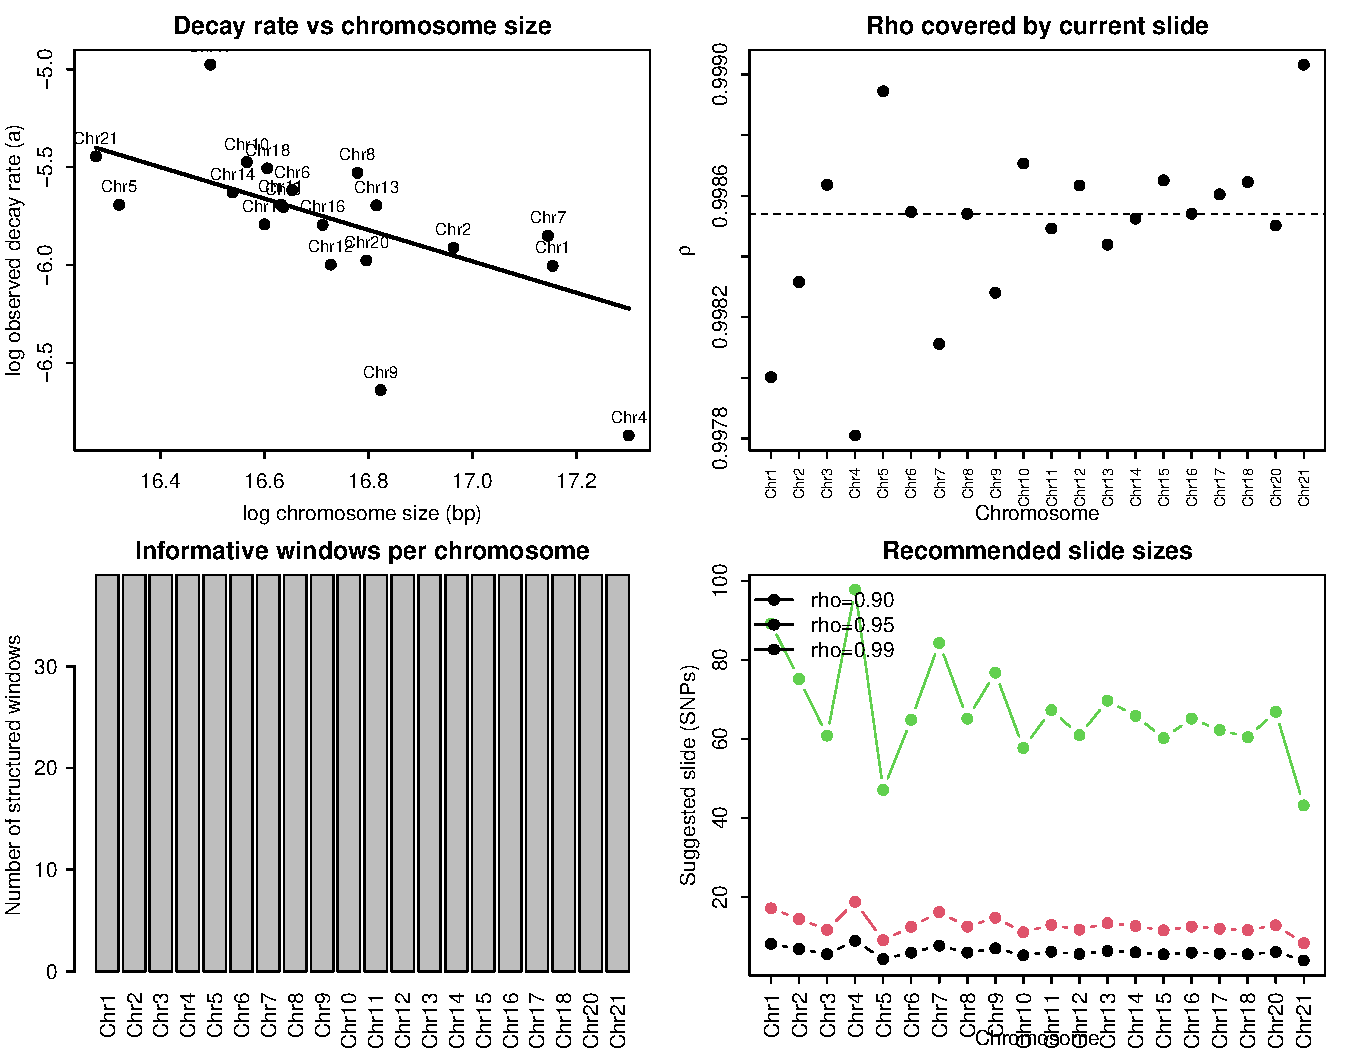
\includegraphics[width=0.85\textwidth,page=1]{figures/decay_curves_example.pdf}
\caption{\code{decay_curves.pdf}, page 1 (genome-wide summary), for
\code{full_runs/3sp_full}: decay rate vs.\ chromosome size (a real
regression across all 20 chromosomes, not the flat line the two-chromosome
worked example would show), LD retained by the current \code{slide}
setting, and informative windows per chromosome. Each chromosome then gets
its own page (not shown) with its window-wise fit against the pooled data.}
\label{fig:decay-curves}
\end{figure}

\subsection{Structure-alignment diagnostic}
\label{sec:alignment}

\textbf{Function:} \code{check_structure_alignment(dataset_dir, cfg)}.
\textbf{Runs when:} \code{input/population.rds} exists.
\textbf{Writes:} \code{output/alignment/}.

Before any association test runs, this asks how much of the tested
phenotype is already explained by population structure --- specifically, by
(a) \code{structure_group.rds} (the sampling groups a permutation null
would shuffle within) and (b) the leading axes of the population-level GRM.
\textbf{This is a warning diagnostic, not a gate}: a low alignment does not
invalidate a result, but a high one means the phenotype and ancestry provide
nearly interchangeable explanations for whatever signal Stage A finds, and
that is worth knowing before interpreting a hit.

\subsubsection*{\code{observed.csv} --- one row}

\begin{Verbatim}
n_individuals n_populations n_structure_groups grm_axes_r2_population
          117            35                  4              0.1033205
grm_axes_adjusted_r2_population structure_r2_population
                     -0.05127941               0.0541958
structure_r2_individual_weighted
                        0.1113596
\end{Verbatim}

\begin{longtable}{@{}L{4.6cm}L{9.9cm}@{}}
\toprule
\textbf{Column} & \textbf{Meaning} \\
\midrule
\endhead
\code{n_individuals}, \code{n_populations}, \code{n_structure_groups} &
  Sample sizes: individuals, distinct \code{population.rds} values, distinct
  \code{structure_group.rds} values. \\
\code{grm_axes_r2_population} & $R^2$ of population-mean phenotype
  regressed on the top eigenvectors of the population-level GRM. \\
\code{grm_axes_adjusted_r2_population} & The same, adjusted $R^2$
  (penalised for the number of axes used). \\
\code{structure_r2_population} & $R^2$ of population-mean phenotype
  regressed on \code{structure_group}, weighted one point per population. \\
\bcode{structure\_r2\_individual\_weighted} & The same, weighted one point
  per individual (populations with more individuals count more). \\
\bottomrule
\end{longtable}

\subsubsection*{\code{null_draws.csv} --- one row per (scheme, draw)}

Every draw's own version of \code{observed.csv}'s three measures,
recomputed on a null-shuffled/null-surrogate phenotype. Two null schemes are
used: \code{"within-group permutation"} (shuffle within
\code{structure_group}) and \code{"GRM-matched continuous"} (a continuous
surrogate matched to the GRM's own covariance structure).

\begin{Verbatim}
                    scheme  draw grm_axes_r2_population structure_r2_population
1 within-group permutation     1              0.09180002               0.0541958
2 within-group permutation     2              0.11839943               0.0541958
3 within-group permutation     3              0.15230749               0.0541958
   structure_r2_individual_weighted
1                        0.03626990
2                        0.22767224
3                        0.12800670
\end{Verbatim}

\subsubsection*{\code{null_summary.csv} --- one row per (scheme, metric)}

\code{observed.csv}'s three measures compared against their own null
distribution.

\begin{Verbatim}
                   scheme                          metric  observed null_mean
within-group permutation          grm_axes_r2_population 0.1033205 0.1300955
  GRM-matched continuous          grm_axes_r2_population 0.1033205 0.3044517
within-group permutation         structure_r2_population 0.0541958 0.0541958
  null_median      null_sd  null_q025 null_q975 observed_within_null95
   0.1197442 5.714492e-02 0.04991410 0.2674327                   TRUE
   0.2924182 1.443470e-01 0.07612137 0.6073546                   TRUE
   0.0541958 1.039326e-16 0.05419580 0.0541958                   TRUE
   proportion_null_ge_observed
                          0.630
                          0.931
                          1.000
\end{Verbatim}

\begin{longtable}{@{}L{3.6cm}L{10.9cm}@{}}
\toprule
\textbf{Column} & \textbf{Meaning} \\
\midrule
\endhead
\code{scheme}, \code{metric} & Which null, and which of the three measures. \\
\code{observed} & The observed value (from \code{observed.csv}). \\
\code{null_mean}, \code{null_median}, \code{null_sd} & That null
  distribution's own summary. \\
\code{null_q025}, \code{null_q975} & The null's 2.5th/97.5th percentile. \\
\bcode{observed\_within\_null95} & Whether \code{observed} falls inside
  $[\code{null_q025}, \code{null_q975}]$ --- if \code{TRUE}, the observed
  alignment is not distinguishable from this null. \\
\bcode{proportion\_null\_ge\_observed} & A one-sided p-value-like quantity:
  the fraction of null draws at least as large as \code{observed}. Low
  values mean the observed alignment is unusually strong relative to this
  null. \\
\bottomrule
\end{longtable}

\subsection{Floor profile: a lightweight sensitivity check on \texttt{size\_floor}}
\label{sec:floor-profile}

\textbf{Function:} \code{run_floor_profile(dataset_dir, targets = c(0.995,
0.997, 0.999))}. \textbf{Runs when:} \code{input/phenotype.rds} exists, by
default (\code{floor_profile = TRUE} in \code{run_dataset()}).
\textbf{Writes:} \code{output/floor_profile/}.

\subsubsection*{Why this exists}

Section~\ref{sec:size-floor-concept} introduced \code{size_floor}: the
minimum Stage-1 cluster size that gets tested at all. Choosing it involves a
real trade-off --- a higher floor tests fewer clusters but covers less of
the genome; a lower floor tests more. Rather than select one integer by
eye, \code{run_floor_profile()} evaluates \emph{three} floors at once,
chosen not by marker count but by how much they actually reduce the number
of tests run: for a candidate integer floor $f$,
\[
\text{reduction}(f) = 1 - \frac{\#\{\text{clusters with } n\_loci \ge f\}}{\#\text{assayed markers}},
\]
and for each target reduction (99.5\%, 99.7\%, 99.9\% by default) the floor
whose achieved reduction is closest is picked. The \emph{middle} target
(99.7\%) is the \textbf{canonical} floor.

\subsubsection*{Only the canonical floor gets the full, permuted treatment}

Running full permutations at three floors instead of one would triple the
cost of the pipeline's most expensive step, which defeats the purpose for a
batch of hundreds of datasets. Instead:

\begin{itemize}
  \item The \textbf{canonical} floor runs Stage A and Stage B exactly as
  \code{run_dataset()} always has --- permutations, the outlier
  permutation test, region assembly --- and \emph{is} the floor
  \code{run_dataset()} adopts as its own \texttt{cfg\$size\_floor} for every
  engine downstream. If the profile is turned off, the separately
  configured \code{size_floor} is used instead.
  \item The two \textbf{side} floors run a fast, \emph{observed-only} pass:
  a floor-specific EMMAX scan with no permutations
  (\code{run_stage_A(permute = FALSE)}) and Stage B's own assembly with no
  permutation-based significance test
  (\code{run_stage_B(observed_only = TRUE)}). This mode does not merely
  skip using a cached permuted null if one exists --- it never attempts to
  load one from disk at all, so a canonical floor's cached permutation
  results can never be picked up by accident.
\end{itemize}

\subsubsection*{How a canonical region's ``stability'' is judged}

A unit's own \code{unit_id} is just a position index into that floor's own
size-filtered cluster list, and is \emph{not} comparable across floors ---
two unrelated clusters can both be ``\code{unit_id} 5'' at two different
floors. Each cluster's \code{core_snp} (Section~\ref{sec:concepts}) is
stable across floors, and is what the floor profile actually keys on to ask
``is this canonical region's cluster \emph{also} a significant unit at
this side floor?''. Physical span overlap is used only as a secondary
sanity check on a recovered hit.

\subsubsection*{Output files}

\code{grid.csv} --- one row per target, on the full 3sp panel (790{,}578
markers, 20 chromosomes):

\begin{Verbatim}
   target floor achieved_reduction n_units_tested marker_coverage is_canonical
1:  0.995     6           0.9955906           3486      0.03854395        FALSE
2:  0.997     7           0.9973500           2095      0.02798712         TRUE
3:  0.999    10           0.9991323            686      0.01435279        FALSE
\end{Verbatim}

\code{summary.csv} --- one compact row per method (\code{unit}/\code{simes}):

\begin{Verbatim}
  method floor_995 reduction_995 floor_997 reduction_997 floor_999 reduction_999
    unit         6     0.9955906         7      0.9973500        10     0.9991323
   simes         6     0.9955906         7      0.9973500        10     0.9991323
  n_units_tested_canonical n_significant_canonical n_regions_canonical
                      2095                     104                  44
                      2095                      73                  35
\end{Verbatim}

\code{canonical_regions_unit.csv} / \code{canonical_regions_simes.csv} ---
one row per \emph{canonical-floor} region (a region found only at a side
floor never appears here --- this table is about how robust the
\emph{reported} findings are, not a census of every floor's own discoveries).
44 rows for the \code{unit} arm on the full 3sp panel; tiers split
18$\times$``3/3'', 23$\times$``2/3'', 3$\times$``1/3'' (a genuine spread,
not the small worked example's near-uniform stability):

\begin{Verbatim}
                region_id    Chr     from       to tick_006 overlap_check_006
Chr1:21492308-21938477   Chr1 21492308 21938477     TRUE              TRUE
Chr7:11386530-11683777   Chr7 11386530 11683777     TRUE              TRUE
Chr12:16941906-17096769  Chr12 16941906 17096769    FALSE                NA
 tick_010 overlap_check_010 n_ticks stability_tier   span
     TRUE              TRUE       3            3/3 446169
     TRUE              TRUE       3            3/3 297247
    FALSE                NA       2            2/3 154863
\end{Verbatim}

\begin{longtable}{@{}L{3.3cm}L{11.2cm}@{}}
\toprule
\textbf{Column} & \textbf{Meaning} \\
\midrule
\endhead
\code{region_id}, \code{Chr}, \code{from}, \code{to}, \code{span} & The
  canonical region's own identity and physical extent. \\
\code{tick_<floor>} & \code{TRUE} if this region's cluster(s) are
  \emph{also} a significant unit at that side floor. A cluster whose
  \code{n_loci} does not clear a side floor is simply never tested there,
  which correctly reads as not-recovered --- this is not a bug, it is what
  floor selection means. \\
\code{overlap_check_<floor>} & Secondary sanity check, only meaningful
  when the tick above is \code{TRUE}: does that side floor's own region
  (containing the recovered cluster) physically overlap this canonical
  region's span? Almost always \code{TRUE}; a \code{FALSE} here is a
  genuine anomaly worth a manual look. \\
\code{n_ticks}, \code{stability_tier} & How many of the 3 floors
  (canonical + 2 side) found this region: \code{"3/3"}, \code{"2/3"}, or
  \code{"1/3"} (never \code{"0/3"}, since every row starts from a
  canonical, already-found region). \\
\bottomrule
\end{longtable}

\textbf{This is a descriptive robustness label, not a significance
measure} --- never a p-value, an FDR estimate, or an independent
replication. A region that persists across floors can still be generated
by population structure. Only the canonical floor's regions get the structure-aware
permutation null; a ``3/3'' region has not been separately re-tested against
a null at the other two floors, it has simply \emph{also} cleared
multiple-testing correction there.

There is empirical reason to use the label as a ranking aid: in 600 primary
simulations with known causal variants, the fraction of reported regions
matching a detectable causal variant increased from 0.317 to 0.524 to
0.692 across one-, two- and three-setting support for the EMMAX consensus
analysis. This does not make a tier a calibrated probability of truth in a
new dataset; demographic structure can produce stable candidates too.

\subsection{The heavier alternative: \texttt{run\_floor\_sweep()}}

\textbf{Function:} \code{run_floor_sweep(dataset_dir, factors = c(0.5, 1,
2))}. Not run by default inside \code{run_dataset()}.

Where the floor profile above deliberately keeps two of its three floors
cheap (observed-only), \code{run_floor_sweep()} reruns \emph{full}
permutations at every floor it tests (half/default/double the resolved
\code{size_floor}). This is a genuinely more expensive, more thorough
robustness check, appropriate for a one-off analysis of a single dataset,
not for a batch of hundreds. Call it separately when you want that extra
assurance.

\code{floor_sweep_summary.csv} --- one row per (floor, statistic):

\begin{Verbatim}
   floor statistic n_units_tested n_significant n_regions
       8      unit            337            62        13
       8     simes            337            51         9
\end{Verbatim}

\begin{longtable}{@{}L{3.4cm}L{11.1cm}@{}}
\toprule
\textbf{Column} & \textbf{Meaning} \\
\midrule
\endhead
\code{floor} & The resolved integer \code{size_floor} this row used. \\
\code{statistic} & \code{"unit"} or \code{"simes"}. \\
\code{n_units_tested} & How many units cleared this floor and were
  tested. \\
\code{n_significant} & How many of those were significant at \code{alpha}. \\
\code{n_regions} & How many regions the significant units assembled
  into. \\
\bottomrule
\end{longtable}

\subsection{Stage A: EMMAX association testing}
\label{sec:stage-a}

\textbf{Function:} \code{run_stage_A(dataset_dir, cfg)}.

\textbf{Writes:} the \code{emmax_unit} and \code{emmax_simes}
subfolders of \code{output/pvalues/}.

Both arms use the same EMMAX mixed model (genotypes, phenotype, the GRM from
Stage 1) but differ in what gets tested:

\begin{itemize}
  \item \textbf{\code{unit}}: one test per Stage-1 cluster that clears
  \code{size_floor}, using a consensus representation of the cluster's
  member markers (\code{unit_repr = "consensus_dosage"} by default).
  Writes \code{p_obs.rds}/\code{p_perm.rds} (one value per tested unit),
  plus \code{p_obs_marker.rds} --- a genuine, separate per-marker EMMAX
  scan computed purely so this arm's Manhattan plot can show real per-SNP
  variation instead of one flat value repeated across every marker in a
  unit.
  \item \textbf{\code{simes}}: every marker is tested directly, then
  aggregated up to its cluster's p-value via Simes' method --- but only for
  clusters that clear \code{size_floor}. Writes \code{p_obs.rds} for
  \emph{every} marker (needed for full-resolution plotting regardless of
  what is actually tested) and \code{p_perm_compact.rds}, a permutation
  matrix restricted to markers whose cluster clears the floor. At
  full-genome scale this restriction is the single biggest cost saving in
  the whole pipeline: on the full 3sp panel, only 16{,}890 of 790{,}578
  markers (2.1\%) sit in a cluster clearing \code{size_floor = 8}, so
  rescanning the other 97.9\% on every permutation would be pure waste.
\end{itemize}

These outputs are R objects (\code{.rds}), not tables to preview here ---
Section~\ref{sec:stage-b} shows what they turn into once Stage B reads them.

\subsection{Stage B: LD-aware outlier detection}
\label{sec:stage-b}

\textbf{Function:} \code{run_stage_B(dataset_dir, engine, cfg)}, once per
available engine. \textbf{Writes:} \code{output/stageB_<engine>/}.

This is where a vector of per-marker p-values becomes a decision: which
clusters are significant, and which physically contiguous regions do they
assemble into. Engine-agnostic by design --- Stage A's own \code{emmax_unit}
and \code{emmax_simes} arms, and any \code{external_pvalues/*.rds} file,
go through the identical call. \code{full_runs/3sp_full} demonstrates this
directly: it has an \code{external_pvalues/lfmm.rds}, so its Stage B runs
three times (\code{emmax_unit}, \code{emmax_simes}, \code{lfmm}) --- compare
the \code{lfmm} region table below (57 regions) against \code{emmax_unit}'s
(44 regions): same columns, same meaning, from a completely different
upstream method, over the same 790{,}578-marker panel.

\subsubsection*{\code{snp_results.csv} --- one row per marker in \code{map}}

The first five rows of \emph{any} panel are mostly \code{NA}, since most
markers are not tested; a filtered view (\texttt{tested == TRUE \&
significant == TRUE}) is more informative:

\begin{Verbatim}
        marker  Chr      Pos statistic marker_p marker_q      unit_p     unit_q
Chr1:19374296 Chr1 19374296      unit       NA       NA 0.002316167 0.04711038
Chr1:19374302 Chr1 19374302      unit       NA       NA 0.002316167 0.04711038
 p_display  q_display unit_id              region_id significant tested   ld_w_095
0.10035796 0.87447990      90 Chr1:19374296-19374576        TRUE   TRUE 0.03257659
0.04846713 0.81744030      90 Chr1:19374296-19374576        TRUE   TRUE 0.02403367
\end{Verbatim}

\begin{longtable}{@{}L{3.0cm}L{11.5cm}@{}}
\toprule
\textbf{Column} & \textbf{Meaning} \\
\midrule
\endhead
\code{marker} & Marker ID, from \texttt{map\$marker}. \\
\code{Chr}, \code{Pos} & Chromosome and position, from \code{map}. \\
\code{statistic} & \code{"unit"} or \code{"simes"} (or whatever
  \code{statistic} an external engine was run with) --- which arm produced
  this row. \\
\code{marker_p}, \code{marker_q} & The marker's own raw p-value / BH
  q-value. Only meaningful when \code{p_obs} is marker-aligned
  (\code{statistic = "simes"}, or any external engine); \code{NA} for
  \code{statistic = "unit"}, where no per-marker p-value exists at all. \\
\code{unit_p}, \code{unit_q} & The marker's tested unit's p-value/q-value,
  broadcast to every member marker. This is what \code{significant} is
  decided from, for \emph{both} statistics. \\
\code{p_display}, \code{q_display} & What the Manhattan plot
  (Section~\ref{sec:manhattan}) actually plots. Identical to
  \code{marker_p}/\code{marker_q} when those exist; for \code{statistic =
  "unit"}, the separate per-marker EMMAX scan mentioned in
  Section~\ref{sec:stage-a} (\code{p_obs_marker.rds}) --- distinct from
  the flat broadcast \code{unit_p}, so the ``unit'' engine's plot still
  shows real per-SNP variation instead of one flat value per cluster. \\
\code{unit_id} & Which Stage-1 cluster (that cleared \code{size_floor})
  this marker belongs to, or \code{NA} if the marker's cluster did not
  clear the floor (never tested). \\
\code{region_id} & Which assembled region this marker's unit belongs to,
  or \code{NA} if its unit was not significant / not assembled into any
  region. String form \code{"<Chr>:<from>-<to>"}. \\
\code{significant} & Whether this marker's unit cleared \code{alpha} after
  BH correction. \code{NA} when \code{tested} is \code{FALSE}. \\
\code{tested} & Whether this marker's unit cleared \code{size_floor} and
  was actually tested (equivalent to \code{!is.na(unit_id)}). \\
\code{ld_w_095} & Local-LD support at $\rho=0.95$
  (Section~\ref{sec:ldw-concept}), carried from \code{map}. Identical
  across every engine's \code{snp_results.csv} for this dataset --- it is
  not a property of any one test. \\
\bottomrule
\end{longtable}

\emph{Note on membership.} Assignment to \code{unit_id}/\code{region_id} is
by exact cluster/group membership, never by whether a marker's coordinate
merely falls inside a region's bounding span. Stage-1 clusters, and the
groups region assembly merges them into, are not necessarily contiguous, so
a wide region span can physically contain markers that actually belong to a
different, interleaved cluster.

\subsubsection*{\code{region_table.csv} --- one row per assembled region}

\begin{Verbatim}
   Chr     from       to n_units n_markers occupancy
  Chr1 19374296 19374576       1        10 0.5263158
  Chr1 21492308 21938477      47      1375 0.5517657
  Chr1 26932748 26932776       1         7 1.0000000
\end{Verbatim}

\begin{longtable}{@{}L{2.6cm}L{11.9cm}@{}}
\toprule
\textbf{Column} & \textbf{Meaning} \\
\midrule
\endhead
\code{Chr}, \code{from}, \code{to} & The region's genomic span (bp). \\
\code{n_units} & How many of this engine's significant units were
  assembled into this region. \\
\code{n_markers} & How many markers belong to this region's own assembled
  units (or group). \\
\code{occupancy} & \code{n_markers} divided by how many markers on
  \code{map} physically fall within \code{[from, to]}. 1.0 means every
  marker in the region's own physical span actually belongs to it; lower
  values mean other, unrelated markers are interleaved within the same
  bounding box --- a lower-occupancy region is a looser, less contiguous
  signal. \\
\bottomrule
\end{longtable}

\subsubsection*{\code{report.txt}}

\code{LDscnR}'s own console summary methods
(\code{print.ld_outlier_test()}, \code{print.ld_outlier_perm()},
\code{print.ld_region_rotation()}), captured verbatim --- no separate
summary logic of this repository's own:

\begin{Verbatim}
<ld_outlier_test> unit / stage2_discovered | floor = 7, alpha = 0.05 | 104/2095 units -> 44 regions

<ld_outlier_perm> observed 104 | surrogate mean 2.71 | p = 0.0020 | null/obs ratio 2.6%
\end{Verbatim}

The nine-spine panel's own \code{report.txt} (\code{full_runs/9sp_full}) is a
useful contrast: 110 significant units out of 3{,}498 tested, but the
permutation test itself is \emph{not} significant overall (surrogate mean
86.62, close to the 110 observed) --- a reminder that many individually
BH-significant units do not automatically mean the panel-wide consensus test
is significant; the two are asking different questions.

\begin{Verbatim}
<ld_outlier_test> unit / stage2_discovered | floor = 11, alpha = 0.05 | 110/3498 units -> 73 regions

<ld_outlier_perm> observed 110 | surrogate mean 86.62 | p = 0.2727 | null/obs ratio 78.7%
\end{Verbatim}

\subsection{Manhattan plots}
\label{sec:manhattan}

\textbf{Function:} \code{ldm_manhattan(dataset_dir, engines, value)}.

\textbf{Writes:} Manhattan plots in \code{output/figures/}, showing either
association q-values or the local LD measure \code{ld_w_095}. The latter
lets a reported region be compared with the local LD pattern; it is not a
second association test.

One panel is drawn per available engine, stacked on a single shared,
continuous genome-wide x-axis (chromosomes concatenated, not faceted, with
alternating light-grey bands marking where each chromosome starts and
ends). Non-significant markers are always a grey background layer;
significant markers are coloured by their assembled region, using a locally
contrastive colour assignment so that two physically nearby regions are
never given confusingly similar hues. The most significant regions per
panel are labelled directly (not via a legend); whenever a floor profile
(Section~\ref{sec:floor-profile}) has been run for that engine's statistic,
the label also carries its stability tier, e.g.\ \code{"R5 (3/3)"}.

\begin{figure}[htbp]
\centering
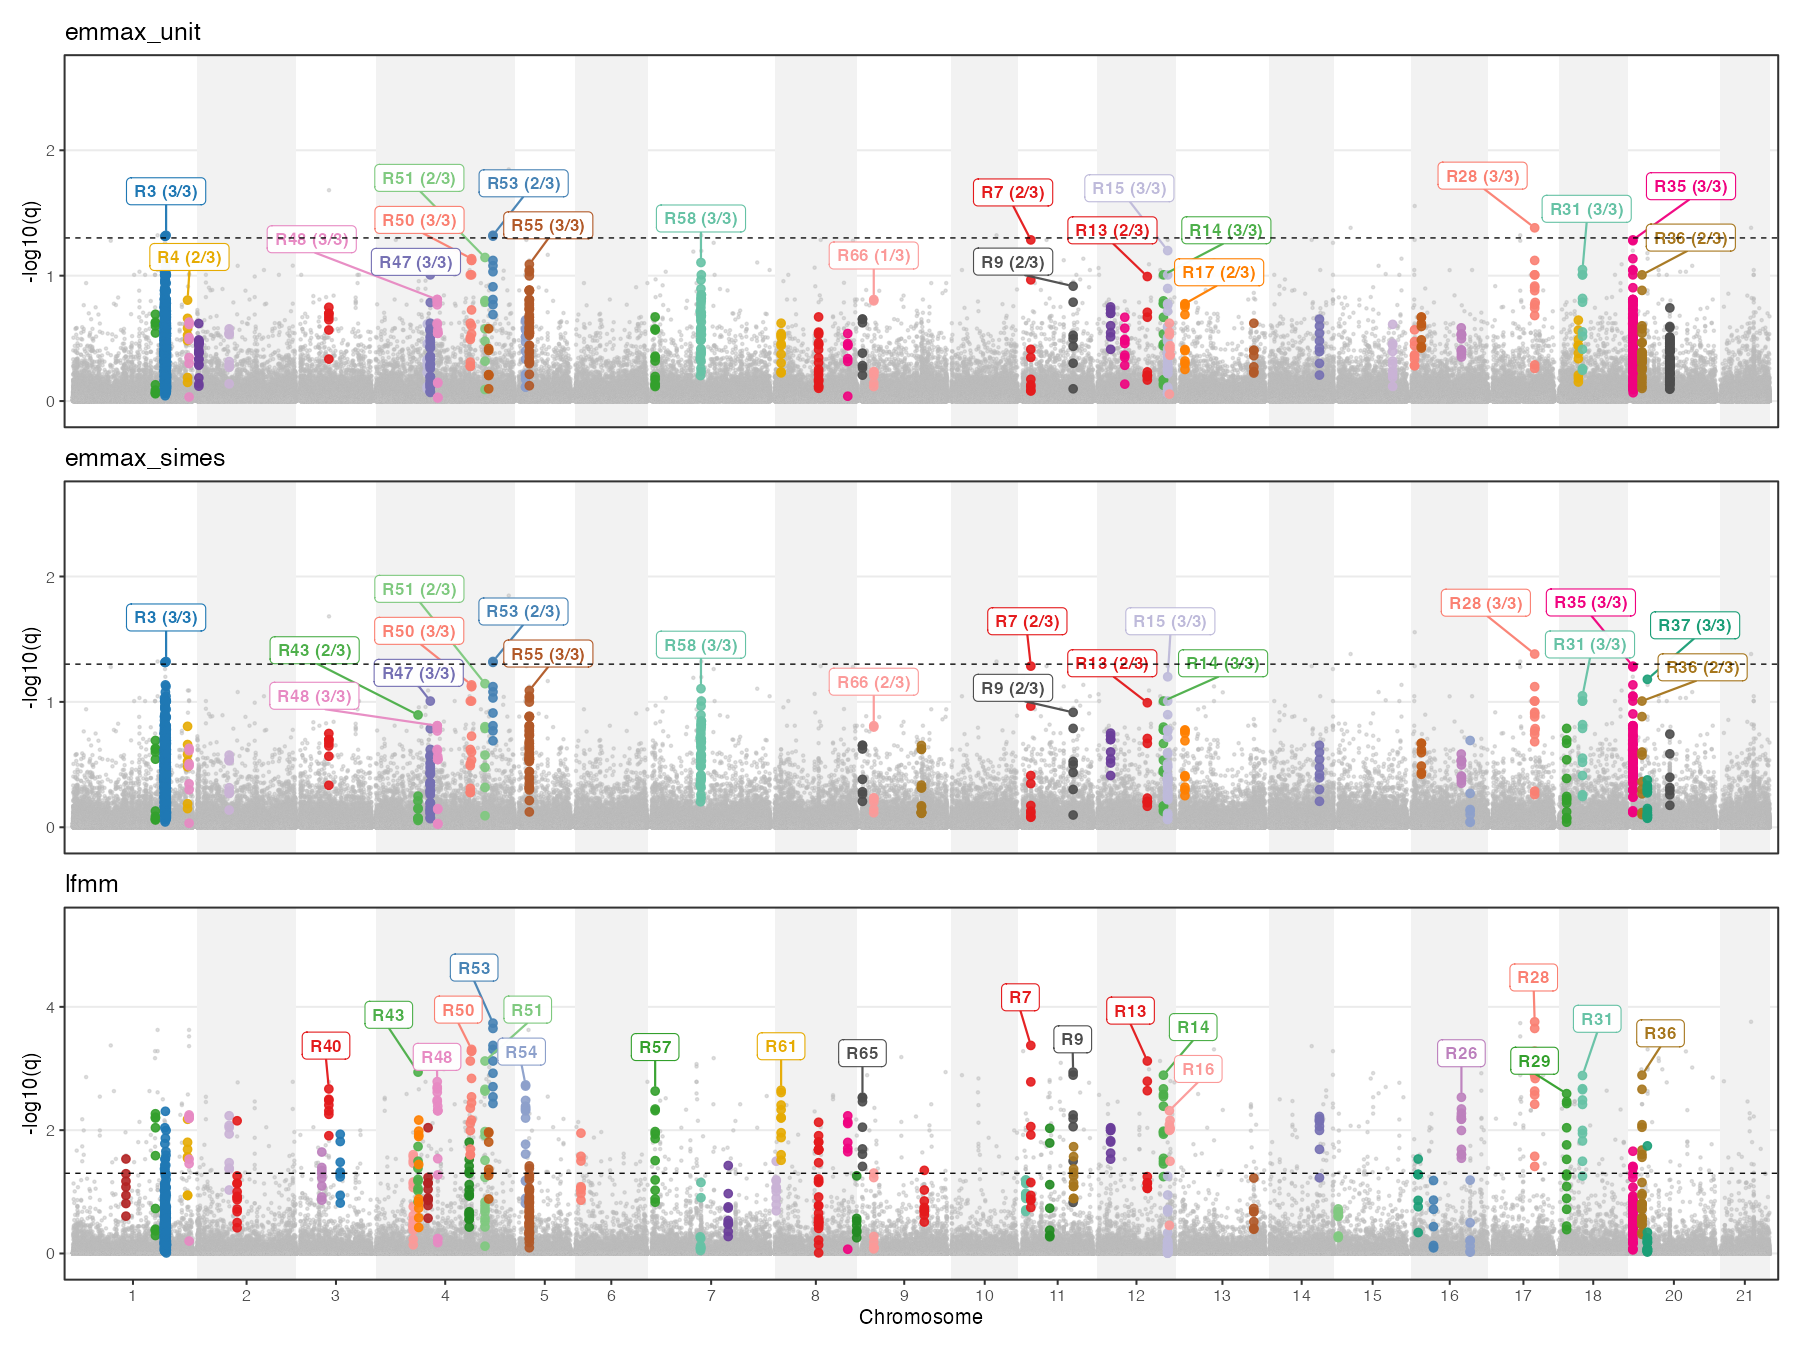
\includegraphics[width=\textwidth]{figures/manhattan_example.png}
\caption{\code{output/figures/manhattan.png} for \code{full_runs/3sp_full}
(full genome, 20 chromosomes) --- q-value on the y-axis, one panel per engine
(\code{emmax_unit}, \code{emmax_simes}, \code{lfmm}), stability tiers shown
on the two EMMAX panels.}
\label{fig:manhattan-q}
\end{figure}

\begin{figure}[htbp]
\centering
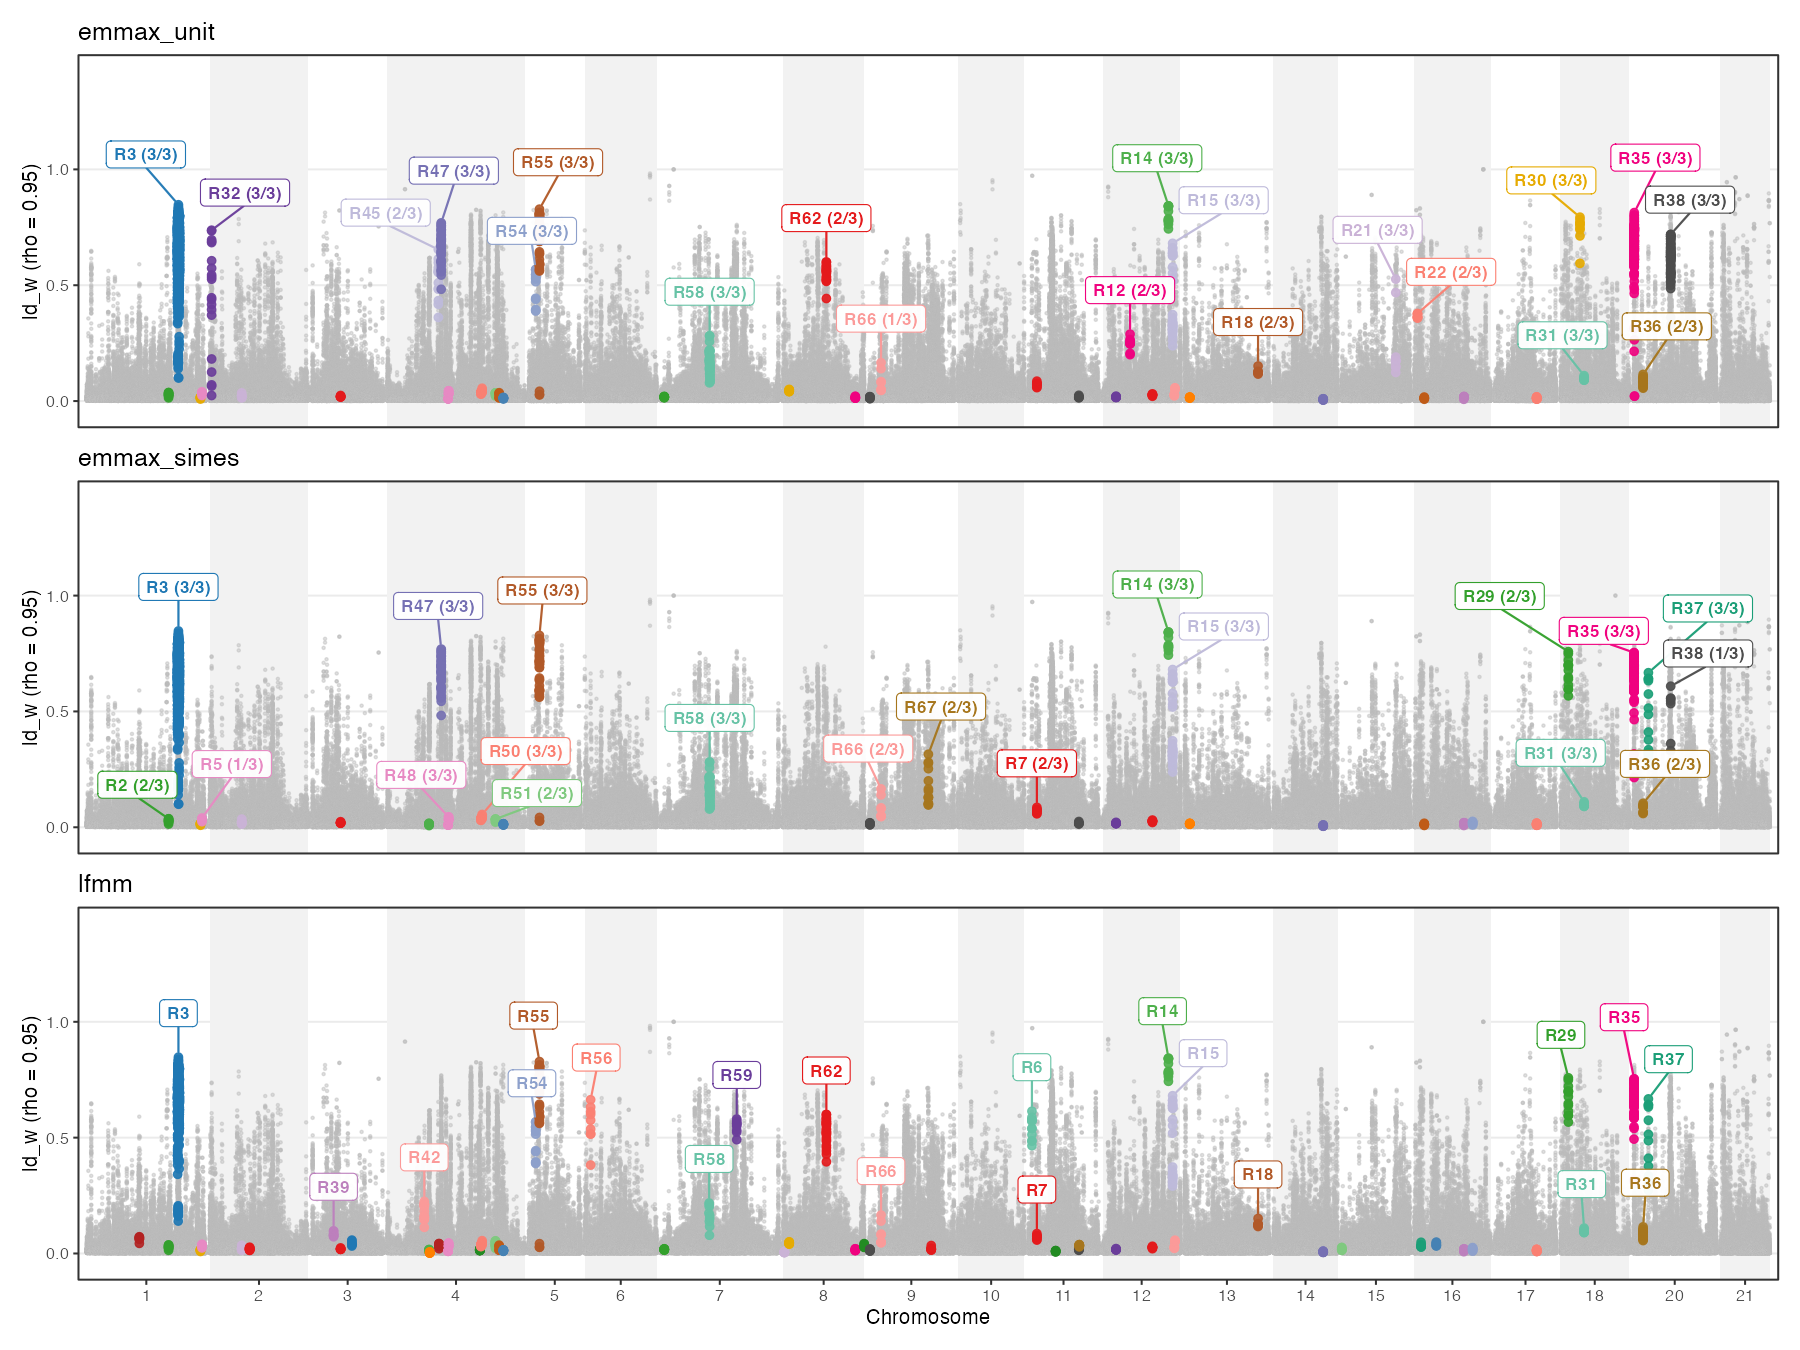
\includegraphics[width=\textwidth]{figures/manhattan_ldw_example.png}
\caption{The same dataset, same panels, \code{ld_w_095} on the y-axis
instead of q-value.}
\label{fig:manhattan-ldw}
\end{figure}

% =============================================================================
\section{Batch summary: \texttt{run\_all()}}
% =============================================================================

\textbf{Function:} \code{run_all(dataset_dirs)}. Loops
\code{run_dataset()} over every folder, isolates one dataset's failure from
the rest (recorded as \code{status = "error"}, not an abort), and writes two
roll-up CSVs at the top level.

\subsubsection*{\code{summary.csv} --- one row per (dataset, engine)}

\begin{longtable}{@{}L{3.6cm}L{11.5cm}@{}}
\toprule
\textbf{Column} & \textbf{Meaning} \\
\midrule
\endhead
\code{dataset} & \code{basename(dataset_dir)}. \\
\code{engine} & Which p-value engine this row is for (\code{emmax_unit},
  \code{emmax_simes}, or an external engine's name). \code{NA} if the
  dataset had no engine to run, or errored before reaching one. \\
\code{n_markers} & Total markers in this dataset's \code{map}. \\
\code{n_units_tested}, \code{n_significant}, \code{n_regions} & Same
  meaning as \code{floor_sweep_summary.csv}'s columns, for this engine's
  actual (non-swept) run. \\
\code{runtime_s} & Wall-clock seconds for this dataset's whole
  \code{run_dataset()} call --- shared across every engine row for that
  dataset, not per-engine timing. \\
\code{status} & \code{"ok"}, \code{"no_engine"} (ran, but had no p-value
  source), or \code{"error"}. \\
\code{error} & The error message, when \code{status = "error"}; \code{NA}
  otherwise. \\
\code{align_grm_axes_r2}, \code{align_grm_axes_p},
  \code{align_structure_r2}, \code{align_structure_p} & The two
  headline structure-alignment numbers, repeated onto every engine row for
  this dataset so a screen of many datasets can sort/filter on association
  results and confounding risk at once. All \code{NA} when the dataset has
  no \code{input/population.rds}. \\
\bottomrule
\end{longtable}

The four \code{align_*} columns use only the ``within-group permutation''
null scheme. \code{align_grm_axes_r2} and \code{align_structure_r2} are
that metric's \code{observed} value; \code{align_grm_axes_p} and
\code{align_structure_p} are its \code{proportion_null_ge_observed} ---
low values flag a phenotype whose signal is hard to distinguish from
ancestry/sampling structure alone.

\code{alignment_summary.csv} is the detailed companion, one row per dataset
with \code{input/population.rds}: \code{dataset}, then every
\code{observed.csv} column, then three columns per (scheme, metric) pair
from \code{null_summary.csv}, named as follows (\code{scheme} with any
non-alphanumeric characters collapsed to \code{_}):

\begin{Verbatim}[fontsize=\footnotesize]
<scheme>__<metric>__null_mean
<scheme>__<metric>__observed_within_null95
<scheme>__<metric>__proportion_null_ge_observed
\end{Verbatim}

% =============================================================================
\section{Configuration reference}
\label{sec:config-reference}
% =============================================================================

Precedence: \code{R/00_config.R}'s \code{DEFAULTS} $<$ a dataset's own
\code{input/config.R} $<$ an explicit \code{cfg =} argument at the call
site.

\begin{longtable}{@{}L{2.6cm}L{3.6cm}L{7.9cm}@{}}
\toprule
\textbf{Name} & \textbf{Default} & \textbf{Meaning} \\
\midrule
\endhead
\code{cr_rho} & 0.5 & LD threshold for Stage-1 clustering
  (\code{ld_complexity_reduction()}). \\
\bcode{decay\_args\$slide} & 450 & Window size (in SNPs) for the raw
  pairwise edge list every LD computation builds per chromosome. Calibrated
  down from \code{compute_LD_decay()}'s own default of 1000 specifically
  to keep the on-the-fly rebuild (see \code{cache/}, Section~\ref{sec:dataset-contract})
  small at full-genome marker density; verified not to move \code{ld_w}
  meaningfully relative to a larger window. \\
\bcode{decay\_args} (other fields) & see \code{R/00_config.R} & The
  remaining LD-decay fitting parameters (MAF filter, background-LD
  quantile, subsampling sizes, robust-fit probability, number of decay
  windows, \ldots) --- see \code{decay_summary.csv}'s glossary
  (Section~\ref{sec:ld-decay}) for what they feed into. \\
\code{statistics} & \bcode{c("unit","simes")} & Which Stage-A arm(s) to
  compute. \\
\bcode{unit\_repr} & \bcode{"consensus\_dosage"} & How a Stage-1 cluster's
  member markers are collapsed into one representation for the ``unit''
  arm. \\
\bcode{grm\_method} & \code{"GCTA"} & \code{SNPRelate::snpgdsGRM()} method
  used to build the genomic relationship matrix. \\
\code{b_unit} & 1000 & Permutations for the ``unit'' arm. \\
\code{b_simes} & 200 & Permutations for the ``simes'' arm (more expensive
  per permutation, since every eligible marker is rescanned). \\
\bcode{size\_floor} & \code{NULL} (derived) & Minimum tested cluster size ---
  see Section~\ref{sec:size-floor-concept}. With the default floor profile
  on, its canonical 99.7\%-reduction floor takes precedence. When that
  profile is off, \code{NULL} derives a floor from marker count; an
  explicit number pins the floor. Always clamped to $\ge 2$. \\
\bcode{size\_floor\_per\_markers} & $10^5$ & Legacy marker-count
  derivation, used only when the floor profile is off and no explicit
  \code{size_floor} was set. \\
\code{alpha} & 0.05 & Significance threshold after BH correction. \\
\bcode{assembly} & \bcode{"stage2\_discovered"} & How significant units are
  merged into regions: a second clustering pass on just the significant
  units (\code{"stage2_discovered"}), or a simple gap-merge of their
  physical spans (\code{"physical"}). \\
\bcode{score\_threshold} & 0.80 & LD threshold used by
  \code{"stage2_discovered"} region assembly. \\
\bcode{distance\_threshold} & $10^5$ & Maximum physical distance (bp)
  \code{"stage2_discovered"} assembly will merge across. \\
\code{gap} & $3\times 10^5$ & Maximum gap (bp) \code{"physical"} assembly
  will merge across. \\
\bcode{n\_rotations} & 10000 & Rotations for \code{ld_region_rotation()}
  (only used when an \code{annotation} is supplied). \\
\bcode{rotation\_scheme} & \code{"within"} & Rotation scheme for the same. \\
\code{seed} & 1 & Random seed. \\
\code{cores} & 1 & Parallel workers for permutation-heavy steps. Increasing
  this forks EMMAX-permutation workers, each holding its own copy of the
  working data --- watch peak memory at high marker counts (see this
  repository's \bcode{full\_runs/*/input/config.R} for a worked example of
  dropping from 8 to 4 after observing memory pressure at 8). \\
\bottomrule
\end{longtable}

% =============================================================================
\section{Caching and receipts}
\label{sec:receipts}
% =============================================================================

Every stage --- Stage 1, Stage A, each Stage B analysis, and the
structure-alignment diagnostic ---
hashes its own inputs and parameters into a \code{_receipt.rds} file next
to its output, and skips recomputing when nothing has changed. These are
\textbf{content} hashes, not timestamps, so a \code{git checkout} or a
copied file cannot produce a false ``unchanged''. Calling
\code{run_dataset()}/\code{run_all()} again on an unchanged dataset is a
cheap no-op walk over receipts. Pass \code{force = TRUE} to any stage
function to rebuild regardless.

A receipt is also treated as stale if a recorded output is missing or the
validated \code{LDscnR} package revision changes. Use \code{force = TRUE}
only when you intentionally want to rebuild results despite unchanged
inputs and settings.

% =============================================================================
\section{Known limitations}
% =============================================================================

\begin{itemize}
  \item \textbf{Plotting at genome scale.} \code{ldm_manhattan()} plots
  every marker by default; Figures~\ref{fig:manhattan-q}--\ref{fig:manhattan-ldw}
  show this works fine at a real, 790{,}578-marker full-genome scale (about
  35 seconds per figure, Section~\ref{sec:running}), but a point-thinning or
  rasterisation pass would still be worth adding for a substantially larger
  panel than this one.
  \item \textbf{One dataset folder per (genotype panel, phenotype) pair.}
  Screening many phenotypes against the same genotype panel currently means
  one folder per phenotype, each independently rebuilding Stage 1
  (genotype-only, and therefore identical across them) and duplicating
  \code{genotypes.rds}/\code{map.rds} on disk. This is fine when ``dataset''
  genuinely means a different genomic panel, but a real cost when it means
  many phenotypes on one panel --- splitting genotype-panel-level shared
  state from phenotype-level per-test state would be a real architecture
  change, not a bolt-on fix.
  \item \textbf{Scope.} Stage B is engine-agnostic on \emph{p-values}, not
  on detection method --- there is no plugin interface for non-\code{LDscnR}
  outlier callers (OutFLANK, BayeScan, pcadapt, \ldots) that a wider
  comparative project might also want to use.
\end{itemize}

% =============================================================================
\appendix
\section{Full output directory tree}
\label{sec:appendix-tree}
% =============================================================================

\begin{Verbatim}
<dataset_dir>/
  input/
    genotypes.rds, map.rds, phenotype.rds, perm_fun.R,
    population.rds, structure_group.rds, config.R
  external_pvalues/
    <engine>.rds                          # one per extra p-value engine
  cache/                                  # gitignored, regenerable
    genotypes.gds, stage1.rds
  output/                                 # gitignored, regenerable
    ld_decay/
      decay_summary.csv, decay_print.txt, decay_curves.pdf
    alignment/
      observed.csv, null_draws.csv, null_summary.csv
    pvalues/emmax_unit/
      p_obs.rds, p_perm.rds, p_obs_marker.rds
    pvalues/emmax_simes/
      p_obs.rds, p_perm_compact.rds
    floor_profile/
      grid.csv, summary.csv,
      canonical_regions_unit.csv, canonical_regions_simes.csv
    stageB_<engine>/
      outlier_test.rds, outlier_perm.rds, region_rotation.rds,
      snp_results.csv, region_table.csv, report.txt
    figures/
      manhattan.png, manhattan.pdf,
      manhattan_ld_w.png, manhattan_ld_w.pdf
    floor_sweep_summary.csv               # only after run_floor_sweep()
    figures/manhattan_floor_sweep.{png,pdf}

<repo root>/
  summary.csv, alignment_summary.csv      # only after run_all()
\end{Verbatim}

\end{document}
